\chapter{Data generation}

In this chapter, we explain how each object in the starGen script is generated. We compare 3D profiles between real and synthetic objects to demonstrate the fidelity of our generator to a real case scenario. We also present examples of each synthetic object and how each parameter affects its appearance. Finally, we explain how synthetic images were generated for the training dataset, and define the parameters used for the generation. 

\subsection{Supported objects}
As already mentioned, the generator supports multiple astronomical objects like stars, galaxies, moving objects, and clusters of moving objects. In this section, we will explain the parameters of each object. 

Note that all number parameters defined by the user are defined in the form of a range, where the user defines the minimum and maximum possible value and the script chooses a specific value from this interval. 

\subsubsection{Stars}
The generator allows user to define the number of generated stars using $count$, their maximal $brightness$, and $fwhm$ of their profile. Stars can be generated either as a point source, where the PSF is Gaussian or as a streak source, which consists of multiple overlapping Gaussians. This is determined by parameter $method$. In case the user chooses the stars to appear as streaks, additional parameters such as their rotation $alpha$ and $length$ need to be set. The rotation $alpha$ is anticlockwise and the values range from 0 to 360 degrees. The length of the streak is measured as half-length and the unit is $\sigma$ of the Gauss function. During one series, stars are static and they stay in the same position. All generated stars have the same $fwhm$, $alpha$ and $length$, while the $brightness$ differs. 

\subsubsection{Moving objects}
Similar to stars user can define the number of moving objects with parameter $count$, their $brightness$, $fwhm$, $method$ of appearance, with the same additional parameters $alpha$ and $length$. However, moving objects are not static and they change positions in consecutive frames. To adjust how much they move in frames, the additional parameter $speed$ was defined. The value of the $speed$ parameter is described as the percentage of the image traveled by the object in one series and it is used in the following manner: 

\begin{equation}
    \Delta = \frac{dim \cdot speed}{frames} 
\end{equation}

where $\Delta$ defines the traveled distance in pixels between two consecutive frames, $dim$ is the smaller dimension of the image, and $frames$ is the number of frames in one series. 

The direction in which the object moves is controlled by the rotation $alpha$ even if the moving object is a point source. The script supports generation of multiple moving objects and each will have different $brightness$, $fwhm$, $alpha$, $length$ and $speed$. 


\subsubsection{Clusters of moving objects}
Clusters are very similar to moving objects and have the same set of parameters. The only difference is that with moving objects when multiple objects are generated each object has different motion parameters ($speed$, $alpha$, and $length$). A cluster object allows multiple objects to have the same motion parameters and move the same way. The number of objects in one cluster is specified with the $objectCountPerCluster$ parameter and each object in the cluster has the same motion. The script supports the generation of multiple clusters with the parameter $count$.   

\subsubsection{Galaxies}
Similar to other objects, the script allows to generate multiple galaxies specifying their number by $count$. Elliptical galaxies have an inner core that is very bright, small, and concentrated. The outer part is larger in the area and the brightness is rapidly fading away from the core. The user can define the brightness of the inner core using the $brightness$ parameter. The brightness of the outer area is calculated using $brightnessFactor$ which defines the percentage of the $brightness$ and is used in the following manner: 

\begin{equation} \label{eq:brightnessGalaxy}
    b_a = brightnessFactor \cdot b_c
\end{equation}

where $b_a$ is the brightness of the outer area, and $b_c$ is the brightness of the core. 
Another parameters include $sigmaX$ and $sigmaY$ that define the variance of the outer area in x, y direction, and $sigmaFactor$ that describes the percentage of the variances for the inner core which is calculated as follows: 

\begin{equation} \label{eq:sigmaGalaxy}
    \begin{split}
        sigmaX_c = sigmaFactor \cdot sigmaX \\
        sigmaY_c = sigmaFactor \cdot sigmaY
    \end{split}
\end{equation}
where $sigmaX_c$, $sigmaY_c$ are variance of the inner core of the galaxy in the x,y direction. 
Lastly, the galaxy has its rotation which is defined by $alpha$ and contains values from 0 to 180 degrees. 


\section{Generated data}
%We have shown how each object is generated and examples of images with just one object. 

The starGen script can generate full-frame series of images with multiple various objects and defects. With the right settings of the configuration file, the system can produce various scenarios mentioned in the Section \ref{sec:scenarios}. Examples of such generated images are shown in the Figure \ref{fig:stargenfullframe}. 

\begin{figure}[!h]
\centering
    \begin{subfigure}[t]{.4\textwidth}
        \centering
        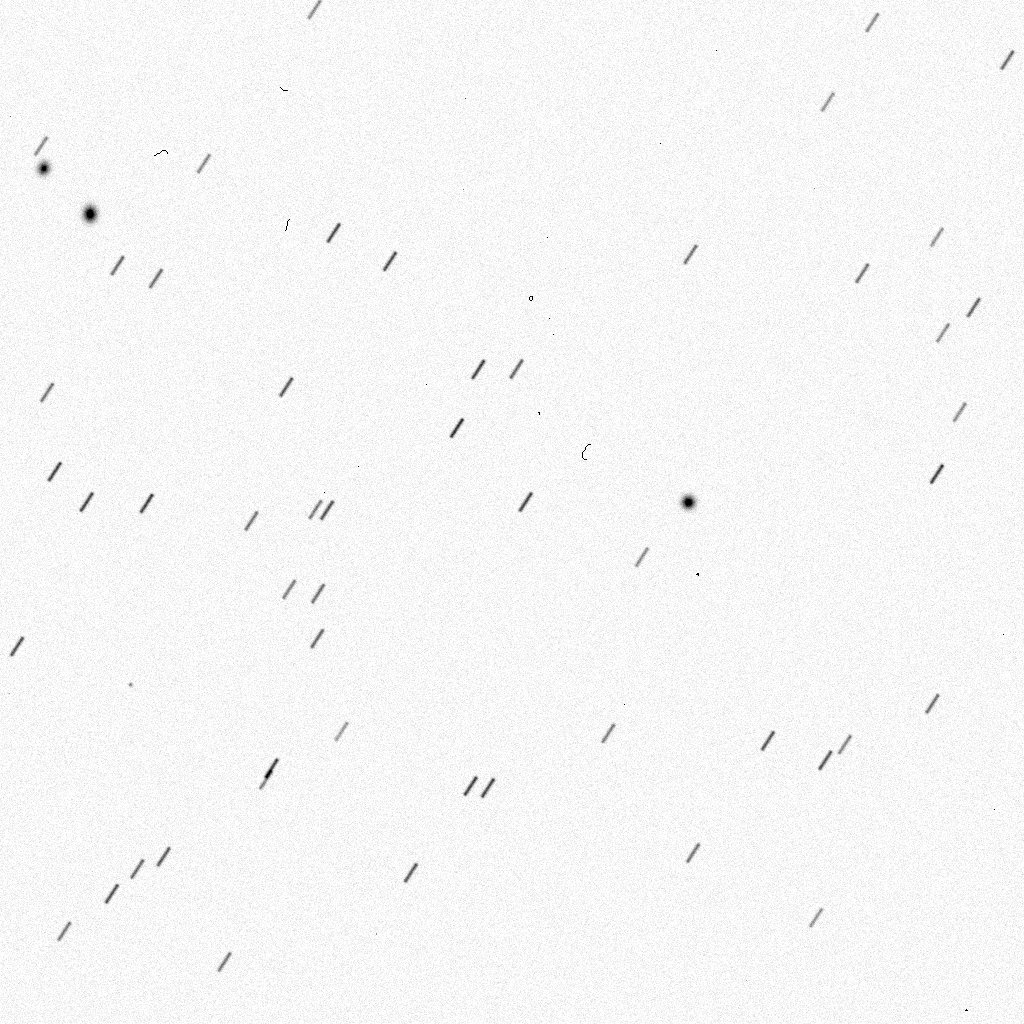
\includegraphics[width=\textwidth]{images/fullframestargen1.jpg}
    \end{subfigure}
    \begin{subfigure}[t]{.4\textwidth}
        \centering
        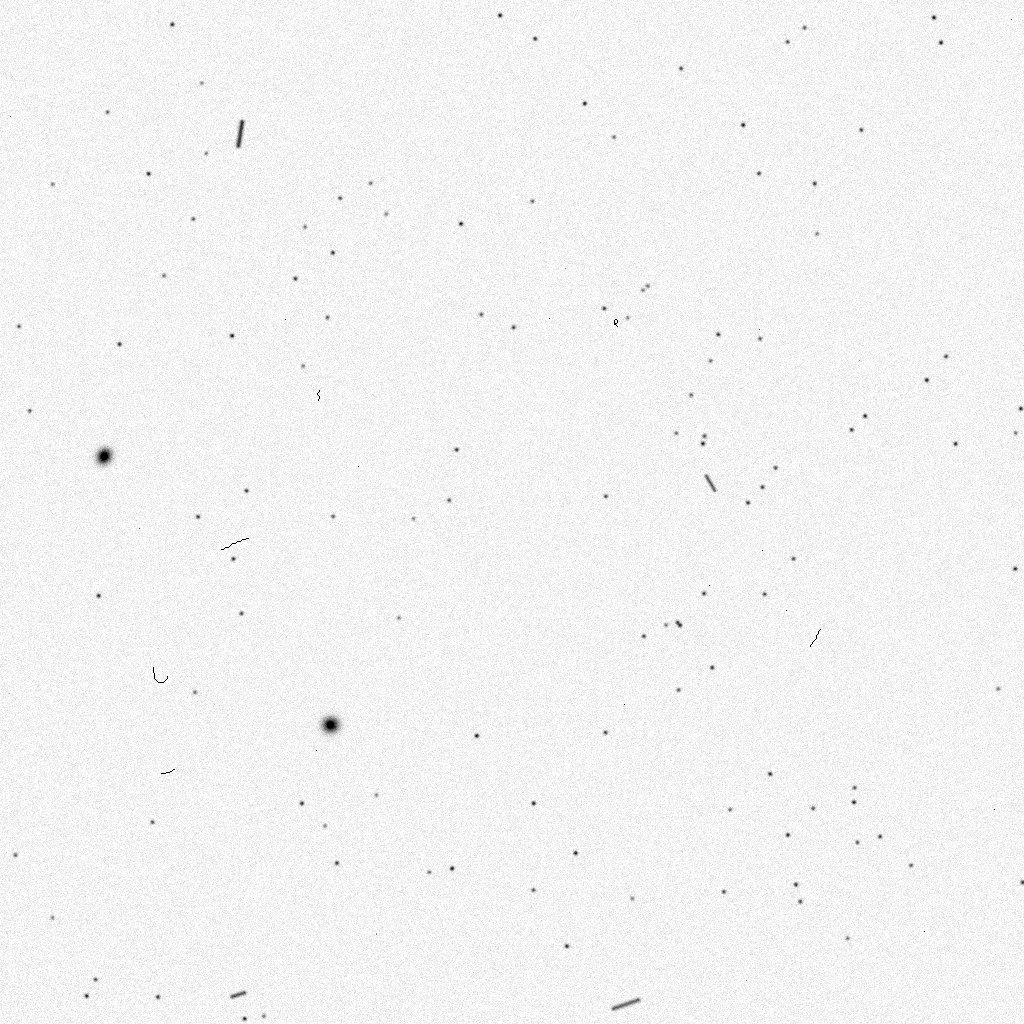
\includegraphics[width=\textwidth]{images/fullframestargen2.jpg}
    \end{subfigure}

    \caption{Synthetic images with a resolution of 1024x1024 generated by starGen.}
    \label{fig:stargenfullframe}
\end{figure}


However, when training the network, we need a 50x50 image with only one object present. To achieve this, we can generate full-frame images and cut out a 50x50 window with one object or we can use starGen to generate images of a given size with just one object. As it was easier to configure the parameters of each object we have decided to generate 50x50 images with one object and produce the training and validation set of data for the network.

Images were generated in 4 iterations, where each iteration represented a degree of brightness of objects. We have generated the following iterations:
\begin{enumerate}
    \item Objects with high brightness (HB)
    \item Objects with medium brightness (MB)
    \item Objects with low brightness (LB)
    \item Objects with very low brightness (VLB)
\end{enumerate}

In the Table \ref{table:bright} we show the brightness range of objects for each iteration. The iteration contains a training and validation set, with objects of the defined brightness. Each iteration could be used independently to train the network. However in our case, after generating all iterations we have merged them together to create the dataset that contains various brightness of objects. 

{\renewcommand{\arraystretch}{1.2}
\begin{table}[h]
\centering
    \begin{tabular}{|l|l|l|}
    \hline
     & \textbf{point, streak, cut streak, galaxy} & \textbf{hot pixels, cosmic rays} \\ \hline
    \textbf{HB}     & <40 000, 60 000>  & <60 000, 65 535> \\ \hline
    \textbf{MB}     & <10 000, 40 000>  & <50 000, 60 000> \\ \hline
    \textbf{LB}     & <2 000, 10 000>   & <10 000, 50 000> \\ \hline
    \textbf{VLB}    & <500, 2 000>      & <2 000, 10 000>  \\ \hline
    \end{tabular}
\caption{Brightness range of generated objects for each iteration.}
\label{table:bright}
\end{table}}


Generating data for the training set, we aimed to have a robust dataset that covers all possible scenarios. For this reason images for the streak, cut streak, and galaxy classes were generated using the Cartesian product of some parameters rather than just choosing randomly from an interval. With streaks, for each $length$ of the streak and each rotation $alpha$, we have generated one image with randomly selected $brightness$ and $fwhm$ from the interval. For both $length$ and $alpha$ the numbers from the interval were selected using an increment of 1. 
%For the length we have selected numbers ranging from 1 to 10 and rotation alpha from 0 to 180 degrees. This gave us a total of 1800 images. 
The same process was followed for cut streaks. 
With galaxies, the Cartesian product of standard deviations $sigmaX$ and $sigmaY$ was used. And for each $sigmaX$ and $sigmaY$ two images were generated, where the other parameters like $alpha$, $brightness$, $brightnessFactor$ and $sigmaFactor$ were selected randomly from the interval. Both standard deviations were selected from the interval with an increment of 0.1. 
%The selected standard deviations were numbers from 1.5 to 4.5 with an increment of 0.1. 
Points, hot pixels, and cosmic rays don't have a lot of parameters to configure, therefore values of parameters were chosen randomly from the interval. However with cosmic rays, for each type, we have generated the same amount of images to keep the dataset balanced. 

Data for the validation set were generated by randomly choosing the value of the parameters from the interval. To preserve the balance of the dataset, each object has the same amount of generated images.

Parameters for each object that were used during the generation of images are depicted in the Table \ref{table:params}. The parameter $brightness$ is not shown in the table since it depends on the data iteration, while the other parameters in the table stay fixed for each iteration. These parameters apply to both the training and validation set. 

{\renewcommand{\arraystretch}{1.2}
\begin{table}[h]
\centering
    \begin{tabular}{|l|l|}
    \hline
    \textbf{Object} & \textbf{Parameters} \\ \hline
    \textit{point} & fwhm = <3.5, 4> \\ \hline
    \textit{streak, cut streak} & \begin{tabular}[c]{@{}l@{}}fwhm = <3.5, 4>\\ length = <1, 10>\\ alpha = <0, 180>\end{tabular} \\ \hline
    \textit{galaxy} & \begin{tabular}[c]{@{}l@{}}alpha = <0, 180>\\ sigmaX = <1.5, 4.5>\\ sigmaY = <1.5, 4.5>\\ brightnessFactor = <0.6, 0.8>\\ sigmaFactor = <0.2, 0.4>\end{tabular} \\ \hline
    \textit{hot pixels} &  \\ \hline
    \textit{cosmic rays} & \begin{tabular}[c]{@{}l@{}}pixelCount = <5, 30>\\ spotPixelCount = <2, 15>\end{tabular} \\ \hline
    \end{tabular}
\caption{Parameter intervals used for the generation of objects.}
\label{table:params}
\end{table}}


To make the generated data look realistic we added various noises. Gaussian noise was applied to each image with $std$ of 100 and $mean$ 200. We also applied Poisson noise to each object. And finally, we used both real DARK and FLAT FIELD frames on our images. Note, that we didn't use the BIAS frame, since the DARK frame we are using already contains the BIAS frame. We have obtained these master frames with a resolution of 1024x1024 pixels, and used the $windowCutter.py$ script to cut 50x50 images. We mentioned in Section \ref{sec:photoreduction} that the DARK frame changes significantly with different exposure times. To account for this, we are using four DARK frames with exposure times of 5, 60, 90, and 360 seconds. For each of these frames, the above-mentioned process of generating objects was used and therefore increasing the amount of data four times, for both training and validation sets.

To sum up, the generated training set for one iteration contains 1800 images for each class, multiplied by 4 DARK frames giving a total of 7200 images per class. After adding all iterations together, the training set consists of 28 800 images per class and a total of 172 800 images. 

For one iteration of the validation set, 1000 images per class were generated. Multiplying by 4 DARK frames gives a total of 4000 images per class. Merging iterations together results in 16 000 images per class for a total of 96 000 images.
